% =====================================================================
% audit_paper_5pp.tex - the submission. "Interpretability as a Science" (NeurIPS 2026 workshop).
%
% STRUCTURE  Introduction -> Background (Fig. 1) -> Related work -> Experimental setup -> Results
%            -> Limitations -> Conclusion. Appendices A-I carry the evidence; references and appendices
%            do not count toward the page limit. Camera-ready, 2026-11-14: de-anonymised and revised
%            for clarity in response to the two reviews; no new results.
%
% ONE DOCUMENT, ON PURPOSE. A 7-page variant and a variant B both existed and were deleted, on
% 2026-08-24 and 2026-08-29. Two documents claiming the same numbers is a currency hazard: the 7pp
% had already drifted once, with a claim-level fix landing in one and not the other.
%
% BUILD      ./build_audit.sh   (regenerates figures and tables, prose gate, compiles, 5-page gate)
% GATE       paper/tools/prose_lint.py paper/audit_paper_5pp.tex --check
%            no em dashes; no bold in the abstract; no hedging boilerplate; sentences under 45 words
% GENERATED  figures/make_audit_figures.py -> figures/f{A,B,D}_*.png
%            paper/tools/make_audit_tables.py    -> tables_audit.tex.  Never edit tables_audit.tex.
%
% FORMATTING RULES, each written down because breaking one cost a revision.
%   - Captions go ABOVE tables, generated ones included. The reader meets the explanation before
%     the grid of numbers, and consecutive appendix tables stop binding to the wrong neighbour.
%   - Appendix tables are [H] and read in source order. Under [h] plus \FloatBarrier they arrived
%     in generator order, pages from their own section, with a third of each page left empty.
%   - A run-in \paragraph heading is a NOUN PHRASE NAMING THE OBJECT of the paragraph. Never an
%     appositive, never a question, never a claim. "Validity, controls and identification" and
%     "Corpora and the containment label" are the form. "The method under study, and its family",
%     "Two aggregations, and what each measures" and "The scale floor, and why it is a precondition
%     rather than a cause" are outline entries, not headings: the "X, and why Y" construction reads
%     as narration and tells the reader nothing they can scan for. The claim goes in the
%     paragraph's FIRST SENTENCE, where the verdict-first rule already puts it. Changed
%     2026-08-30 at Tarush's request, reversing the earlier "heading states the finding as a
%     claim" rule; do not revert without asking.
%   - References start on their own page.
%
% NUMBERS ADDED 2026-08-29, each verified against its results file and not against prose:
%   CV8  results/cv8_positional_extrapolation.json   the positional hedge, retired and bounded
%   E66b results/e66b_determinism_floor.json         the fitter's determinism floor on CUDA
%   E66c results/e66c_post_provenance_repro.json     post-provenance operators reproduce
%   OS1b results/os1b_selfdistance_floor.json        why the operator-space C1 could not have fired
% =====================================================================
\documentclass{article}
% TWO BUILDS FROM THIS ONE SOURCE. Built alone, this file is the workshop camera-ready.
% audit_paper_extended.tex defines \EXTENDED and inputs this file: the public extended version,
% which adds the CV3 score-unit result to App. E (see that file's header). Shared text lives only here.
\ifdefined\EXTENDED
  \usepackage[preprint]{neurips_2026}
\else
  \usepackage[dblblindworkshop,final]{neurips_2026}
\fi
\workshoptitle{Interpretability as a Science}
\ifdefined\EXTENDED
  \makeatletter
  \renewcommand{\@noticestring}{Extended version of a paper at the Interpretability as a Science
    workshop, NeurIPS 2026.}
  \makeatother
\fi

\usepackage[utf8]{inputenc}
\usepackage[T1]{fontenc}
\usepackage{hyperref}
\hypersetup{pdftitle={The Fitting Corpus Is Part of the Measurement: Auditing a Jacobian Lens on Pythia},
  pdfauthor={Tarush Gupta}}
\usepackage{url}
\usepackage{booktabs}
\usepackage{amsfonts,amsmath,amssymb}
\usepackage{nicefrac}
\usepackage{microtype}
\usepackage{xcolor}
\usepackage{array}
\usepackage{enumitem}
\usepackage{graphicx}
\usepackage{float}

% Float packing. LaTeX's stock fractions reserve so much of a float page for the float that a page
% carrying one figure came out with a third of its text height empty.
\renewcommand{\topfraction}{0.92}
\renewcommand{\bottomfraction}{0.85}
\renewcommand{\textfraction}{0.08}
\renewcommand{\floatpagefraction}{0.85}
\setlength{\intextsep}{8pt plus 1pt minus 1pt}
\setlength{\abovecaptionskip}{2pt}
\setlength{\belowcaptionskip}{4pt}
\setlength{\textfloatsep}{10pt plus 2pt minus 4pt}

\newcommand{\mn}{\texttt{min}}
\newcommand{\pe}{\texttt{persist}}
\newcommand{\Jsh}{J^{\mathrm{shuf}}}

\title{The Fitting Corpus Is Part of the Measurement:\\Auditing a Jacobian Lens on Pythia}

\author{%
  Tarush Gupta\\
  Independent Researcher\\
  \texttt{tarushgs@gmail.com}
}

% tables_audit.tex - GENERATED by paper/tools/make_audit_tables.py. Do not edit.
% Every number is read from results/*.json at build time.

\newcommand{\tblladder}{%
\begin{table}[H]
\centering\scriptsize\setlength{\abovecaptionskip}{2pt}\setlength{\belowcaptionskip}{4pt}\setlength{\tabcolsep}{4pt}
\caption{The corpus effect at four rungs of the Pythia ladder. The italic row gives $N$, the number
of fitting prompts per map. $R$ is not comparable across rungs with different $N$, because
the pooled seed SD is $2.29\times$ to $5.70\times$ larger at $N{=}25$ than at $N{=}200$, so the
$N{=}200$ columns and the $N{=}25$ columns are two different scales. The quantity that is comparable
is the $z$ spread, in the last two columns, and it grew from 410M to 2.8B in five of five families.
The 1.4B rung carries no verdict: its numbers were seen before a rule for it could be written. An
$R$ of 10 has a one-sided exceedance of $1.0\times10^{-4}$ to $5.7\times10^{-3}$ under a permutation
null over corpus labels, and $\tau\ge0.6$ has exact null probability $14/120$ per family.}
\label{tab:ladder}
\begin{tabular}{@{}lrrrrrrrrrr@{}}
\toprule
& & \multicolumn{4}{c}{$R$ = spread of $z$ / pooled seed SD} & \multicolumn{3}{c}{Kendall $\tau$ vs.\ 410M}
& \multicolumn{2}{c}{Spread of $z$} \\
\cmidrule(lr){3-6}\cmidrule(lr){7-9}\cmidrule(lr){10-11}
Family & Pairs & 410M & 1B & 1.4B & 2.8B & 1B & 1.4B & 2.8B & 410M & 2.8B \\
& & \emph{200} & \emph{200} & \emph{25} & \emph{25} & & & & \emph{200} & \emph{25} \\
\midrule
Multi-hop & 103 & 25.4 & 29.4 & 7.3 & 11.4 & +0.4 & +0.8 & +0.6 & 0.443 & 0.601 \\
Multilingual & 394 & 19.4 & 25.5 & 7.0 & 14.5 & +0.8 & +1.0 & +0.8 & 0.383 & 0.654 \\
Order of operations & 110 & 24.6 & 31.7 & 4.7 & 6.5 & +0.8 & -0.4 & +0.8 & 0.297 & 0.375 \\
Poetry & 98 & 42.7 & 18.1 & 14.8 & 11.9 & +0.4 & +0.8 & +0.6 & 0.238 & 0.379 \\
Typo & 96 & 27.0 & 23.1 & 16.3 & 11.4 & +0.8 & +0.8 & +1.0 & 0.525 & 0.595 \\
\bottomrule
\end{tabular}

\end{table}}

\newcommand{\tblbaseline}{%
\begin{table}[H]
\centering\small\setlength{\abovecaptionskip}{2pt}\setlength{\belowcaptionskip}{4pt}\setlength{\tabcolsep}{6pt}
\caption{The unfitted baseline rises monotonically at every rung. Any comparison of a fitted
map against the free lens at 2.8B is therefore against a stronger baseline than at 410M, and a
table that omits this row overstates the fitted map at scale.}
\label{tab:baseline}
\begin{tabular}{@{}lrrrr@{}}
\toprule
& 410M & 1B & 1.4B & 2.8B \\
\midrule
Logit-lens readout score, any-layer (\texttt{min}) & 19.81 & 21.90 & 23.94 & 27.00 \\
\bottomrule
\end{tabular}

\end{table}}

\newcommand{\tblfamily}{%
\begin{table}[H]
\centering\scriptsize\setlength{\abovecaptionskip}{2pt}\setlength{\belowcaptionskip}{4pt}\setlength{\tabcolsep}{3.5pt}
\caption{The corpus effect at 410M decomposed by evaluation family. We report per family because
multilingual is $394$ of $801$ scored pairs and the model answers $0.9\%$ of it. The spread is
across the five in-stream fitting corpora; the seed SD is the RMS of per-corpus sample SDs over
three seed blocks, computed inside that family. Wiki is Wikipedia and StackEx is StackExchange. Rank and $z$ disagree about where the effect is largest. The bottom of
the $z$ ordering is the same in all five families; the top three permute. Exploratory.}
\label{tab:family}
\begin{tabular}{@{}lrrrrrrl@{}}
\toprule
Family & Pairs & Logit-lens $z$ & Spread of $z$ & Seed SD & $z$/SD & Rank/SD & Best to worst by $z$ \\
\midrule
Multi-hop & 103 & 3.286 & 0.4426 & 0.01745 & 25.4 & 17.3 & Pile-CC $>$ StackEx $>$ USPTO $>$ Wiki $>$ GitHub \\
Multilingual & 394 & 2.620 & 0.3826 & 0.01970 & 19.4 & 17.9 & StackEx $>$ Pile-CC $>$ USPTO $>$ Wiki $>$ GitHub \\
Order of operations & 110 & 5.086 & 0.2971 & 0.01206 & 24.6 & 29.9 & USPTO $>$ StackEx $>$ Pile-CC $>$ Wiki $>$ GitHub \\
Poetry & 98 & 2.561 & 0.2381 & 0.00558 & 42.7 & 7.3 & Pile-CC $>$ USPTO $>$ StackEx $>$ Wiki $>$ GitHub \\
Typo & 96 & 3.437 & 0.5255 & 0.01945 & 27.0 & 14.7 & StackEx $>$ Pile-CC $>$ USPTO $>$ Wiki $>$ GitHub \\
\bottomrule
\end{tabular}

\end{table}}

\newcommand{\tblderange}{%
\begin{table}[H]
\centering\scriptsize\setlength{\abovecaptionskip}{2pt}\setlength{\belowcaptionskip}{4pt}\setlength{\tabcolsep}{5pt}
\caption{Each fitted map scored against fifteen layer-derangements of itself, at the corrected
readout. Under \texttt{min} seven of eight maps sit below their own null's mean, exact
one-sided binomial $p=0.0352$, and the derangement wins a majority of paired draws on the same seven;
under \texttt{persist} every map sits above its null and the derangement wins none. Fifteen
draws floor the empirical $p$ at $1/16$, so no single row can reach $p<0.05$. The count of maps
clearing every own draw, 0 of 8 under \texttt{min} against 8 of 8 under \texttt{persist}, is not
the inferential statement: a count of zero arises under the exact null with probability
$(15/16)^8=0.597$. The direction is the statistic.}
\label{tab:derange}
\begin{tabular}{@{}lrrrrrrr@{}}
\toprule
& \multicolumn{4}{c}{Any-layer (\texttt{min}), published} & \multicolumn{3}{c}{Majority-layer (\texttt{persist})} \\
\cmidrule(lr){2-5}\cmidrule(lr){6-8}
Fitting corpus & Real & Null mean & $z$ & Null wins & Real & Null mean & $z$ \\
\midrule
Wikipedia & 24.16 & 25.84 & -1.67 & 15/15 & 10.42 & 7.88 & +11.83 \\
USPTO & 26.11 & 26.51 & -0.71 & 12/15 & 12.01 & 8.65 & +12.44 \\
Pile-CC & 26.24 & 27.48 & -1.99 & 15/15 & 11.11 & 8.26 & +15.96 \\
StackExchange & 26.43 & 26.49 & -0.09 & 8/15 & 11.61 & 8.37 & +8.59 \\
GitHub & 24.05 & 23.24 & +0.59 & 5/15 & 10.08 & 8.17 & +7.17 \\
News 2024 & 25.01 & 25.72 & -0.75 & 10/15 & 9.79 & 7.10 & +16.76 \\
arXiv 2023 & 26.93 & 27.03 & -0.09 & 8/15 & 10.59 & 7.92 & +11.74 \\
Common Pile & 25.29 & 26.08 & -0.71 & 11/15 & 10.66 & 7.94 & +16.76 \\
\bottomrule
\end{tabular}

\end{table}}

\newcommand{\tblvariance}{%
\begin{table}[H]
\centering\small\setlength{\abovecaptionskip}{2pt}\setlength{\belowcaptionskip}{4pt}\setlength{\tabcolsep}{5pt}
\caption{Variance shares of the $8\times8$ fit\,$\times$\,read grid at 410M, corrected readout.
Intervals are 95\% bootstrap over both seed factors, 10{,}000 resamples. The ordering holds under
both aggregations, but the interval on the difference excludes zero only under \texttt{min}.}
\label{tab:variance}
\begin{tabular}{@{}lccccc@{}}
\toprule
Recovery rule & Fit \% [95\% CI] & Read \% [95\% CI] & Residual \% & Fit $-$ read [95\% CI] & Excludes 0 \\
\midrule
Any-layer & 53.35 [49.1, 57.0] & 44.61 [41.0, 48.3] & 2.04 & +8.74 [+0.80, +15.87] & Yes \\
Majority-layer & 50.70 [45.2, 54.2] & 48.13 [44.4, 53.0] & 1.17 & +2.57 [-7.60, +9.80] & No \\
\bottomrule
\end{tabular}

\end{table}}

\newcommand{\tblclustered}{%
\begin{table}[H]
\centering\small\setlength{\abovecaptionskip}{2pt}\setlength{\belowcaptionskip}{4pt}\setlength{\tabcolsep}{6pt}
\caption{Corpus-clustered paired $t$ on the derangement gap, the inferential companion to
Table~\ref{tab:derange}. The replication unit is the corpus, not the draw, because fifteen
derangements of one map share the same map and cache. At the corrected readout, evidence that
\texttt{min} prefers the derangement does not clear $5\%$; at the legacy readout it did. We therefore
do not use this null as an identifying control.}
\label{tab:clustered}
\begin{tabular}{@{}llrrr@{}}
\toprule
Scorer & Recovery rule & Mean gap (points) & $t(7)$ & $p$ (two-sided) \\
\midrule
Corrected & Any-layer & -0.522 & -1.92 & 0.096 \\
Corrected & Majority-layer & +2.750 & +17.50 & 4.9e-07 \\
Pre-correction & Any-layer & -1.338 & -3.28 & 0.013 \\
\bottomrule
\end{tabular}

\end{table}}

\newcommand{\tblcompetence}{%
\begin{table}[H]
\centering\small\setlength{\abovecaptionskip}{2pt}\setlength{\belowcaptionskip}{4pt}\setlength{\tabcolsep}{5pt}
\caption{Answer competence, corrected readout, 95\% Wilson intervals~\citep{wilson1927}. Only
multihop, order-ops and multilingual carry an expected answer; poetry, typo and association carry
\texttt{target: null}, so answer competence is undefined for them rather than zero. Prompt surprisal
is the mean per-token negative log likelihood over all 551 items in all six families. Top-1 never
separates from 410M once the intervals are attached, while surprisal falls monotonically: the models
become more fluent on the prompts without becoming measurably better at answering them.}
\label{tab:competence}
\begin{tabular}{@{}lccrrrr@{}}
\toprule
& \multicolumn{2}{c}{Pooled, 255 prompts with an answer} & \multicolumn{3}{c}{Median answer rank}
& Prompt \\
\cmidrule(lr){2-3}\cmidrule(lr){4-6}
Model & Top-1 \% [95\% CI] & Top-10 \% [95\% CI] & Multi-hop & Order of ops. & Multilingual & surprisal \\
\midrule
70M & 1.6 [0.6, 4.0] & 16.9 [12.8, 21.9] & 80 & 18 & 3436 & 5.204 \\
160M & 1.6 [0.6, 4.0] & 22.4 [17.7, 27.9] & 42 & 13 & 3788 & 4.894 \\
410M & 4.7 [2.7, 8.0] & 26.3 [21.3, 32.0] & 31 & 9 & 3044 & 4.374 \\
1B & 4.3 [2.4, 7.6] & 29.4 [24.2, 35.3] & 18 & 7 & 1649 & 4.207 \\
1.4B & 3.1 [1.6, 6.1] & 27.5 [22.3, 33.2] & 24 & 7 & 1345 & 4.106 \\
2.8B & 5.9 [3.6, 9.5] & 32.9 [27.5, 38.9] & 14 & 7 & 578 & 4.013 \\
\bottomrule
\end{tabular}

\end{table}}

\newcommand{\tblposition}{%
\begin{table}[H]
\centering\small\setlength{\abovecaptionskip}{2pt}\setlength{\belowcaptionskip}{4pt}\setlength{\tabcolsep}{5pt}
\caption{Read position against the positional support of the fitted map. The fitter averages
the Jacobian over positions 16 to 126 of a 128-token window. Not one of 551 items
on any prefixed rung is read inside that range, and without a prefix the majority of the remainder
sit below it, inside the attention-sink zone the fitter deliberately excludes. The two conditions
extrapolate in opposite directions.}
\label{tab:position}
\begin{tabular}{@{}lrrrrrrrr@{}}
\toprule
& & Median & \multicolumn{3}{c}{No prefix} & \multicolumn{3}{c}{128-token prefix} \\
\cmidrule(lr){4-6}\cmidrule(lr){7-9}
Family & Prompts & length & Median & Range & In support \% & Median & Range & In support \% \\
\midrule
Association & 102 & 28 & 28 & 19--49 & 100.0 & 156 & 147--177 & 0.0 \\
Multi-hop & 93 & 15 & 15 & 8--40 & 48.4 & 143 & 136--168 & 0.0 \\
Multilingual & 107 & 10 & 10 & 5--26 & 5.6 & 138 & 133--154 & 0.0 \\
Order of ops. & 55 & 8 & 8 & 6--18 & 1.8 & 136 & 134--146 & 0.0 \\
Poetry & 98 & 26 & 18 & 16--22 & 100.0 & 146 & 144--150 & 0.0 \\
Typo & 96 & 8 & 8 & 6--14 & 0.0 & 136 & 134--142 & 0.0 \\
\midrule
All & 551 & & 14 & 5--49 & 45.7 & 142 & 133--177 & 0.0 \\
\bottomrule
\end{tabular}

\end{table}}

\newcommand{\tblcrossover}{%
\begin{table}[H]
\centering\small\setlength{\abovecaptionskip}{2pt}\setlength{\belowcaptionskip}{4pt}\setlength{\tabcolsep}{6pt}
\caption{Each fitted map at 410M against the unfitted logit lens, corrected readout, on
identical cached activations. The readout score is the mean over the five admitted families and three
fitting seeds; the gain is the point estimate relative to the logit lens, whose value is one
number per recovery rule and is printed once. Of the eight differences, 7 under
\mn{} and 2 under \pe{} have three-level hierarchical bootstrap intervals
excluding zero, over eval set, seed block and item pair.}
\label{tab:crossover}
\begin{tabular}{@{}lrrrr@{}}
\toprule
& \multicolumn{2}{c}{Any-layer (\mn)} & \multicolumn{2}{c}{Majority-layer (\pe)} \\
\cmidrule(lr){2-3}\cmidrule(lr){4-5}
Fitting corpus & Readout score & Gain \% & Readout score & Gain \% \\
\midrule
arXiv 2023 & 26.93 & +35.9 & 10.59 & +27.3 \\
StackExchange & 26.43 & +33.4 & 11.61 & +39.6 \\
Pile-CC & 26.24 & +32.5 & 11.11 & +33.6 \\
USPTO & 26.11 & +31.8 & 12.01 & +44.3 \\
Common Pile & 25.29 & +27.6 & 10.66 & +28.2 \\
News 2024 & 25.01 & +26.2 & 9.79 & +17.7 \\
Wikipedia & 24.16 & +22.0 & 10.42 & +25.3 \\
GitHub & 24.05 & +21.4 & 10.08 & +21.1 \\
\midrule
Logit lens (unfitted) & 19.81 & & 8.32 & \\
\bottomrule
\end{tabular}

\end{table}}

\newcommand{\tblcontain}{%
\begin{table}[H]
\centering\small\setlength{\abovecaptionskip}{2pt}\setlength{\belowcaptionskip}{4pt}\setlength{\tabcolsep}{6pt}
\caption{32-gram containment of each fitting corpus against the full published training stream, 20
of 20 shards: the fraction of the corpus's 32-token windows that occur verbatim in the stream. The
five Pile components sit above $0.9$; the three later or external corpora sit at or below the level
that reformatting alone produces (Table~\ref{tab:calib}) and are reported as ``no match found at
$k{=}32$'' rather than as absent from training. The readout each corpus produces is in
Figure~\ref{fig:membership}.}
\label{tab:contain}
\begin{tabular}{@{}llr@{}}
\toprule
Fitting corpus & Group & Containment ($k{=}32$) \\
\midrule
Wikipedia & Pile component & 0.92160 \\
USPTO & Pile component & 0.92676 \\
Pile-CC & Pile component & 0.92761 \\
StackExchange & Pile component & 0.91799 \\
GitHub & Pile component & 0.93400 \\
News 2024 & After the Pile & 0.00075 \\
arXiv 2023 & After the Pile & 0.00009 \\
Common Pile & After the Pile & 0.00125 \\
\bottomrule
\end{tabular}

\end{table}}

\newcommand{\tblcalib}{%
\begin{table}[H]
\centering\small\setlength{\abovecaptionskip}{2pt}\setlength{\belowcaptionskip}{4pt}\setlength{\tabcolsep}{6pt}
\caption{Calibration of the containment index. Re-wrapping identical text to a different line width
leaves only $0.14\%$ to $2.4\%$ of its 32-grams intact, so any value in that band cannot be read as
absence. A post-cutoff Wikipedia dump and a PubMed control both score far above the out-of-stream
corpora, and uniform-random tokens score exactly zero. Document-level temporal exclusion does not
give textual novelty, which is why we report ``no match found at $k{=}32$'' rather than ``absent
from training''.}
\label{tab:calib}
\begin{tabular}{@{}lr@{}}
\toprule
Calibration corpus & Containment ($k{=}32$) \\
\midrule
PubMed (control) & 0.79273 \\
Wikipedia 2023 & 0.26958 \\
FineWeb (trap) & 0.06309 \\
Uniform random tokens & 0.00000 \\
\bottomrule
\end{tabular}

\end{table}}

\newcommand{\tblgrid}{%
\begin{table}[H]
\centering\scriptsize\setlength{\tabcolsep}{3.5pt}
\caption{The 64 cell values behind Figure~\ref{fig:grid}, readout score under
\texttt{min}, corrected readout. Figure~\ref{fig:grid} renders these as colour because the finding
is the row pattern; the margins it prints are the bold row and column means here.}
\label{tab:grid}
\begin{tabular}{@{}lrrrrrrrrr@{}}
\toprule
Fitting corpus & \multicolumn{8}{c}{Read context} & Mean \\
\cmidrule(lr){2-9}
 & Wikipedia & USPTO & Pile-CC & StackExchange & GitHub & News 2024 & arXiv 2023 & Common Pile & \\
\midrule
Wikipedia & 23.90 & 24.36 & 24.11 & 22.11 & 22.36 & 23.87 & 22.41 & 22.10 & \textbf{23.15} \\
USPTO & 26.22 & 26.84 & 26.69 & 24.90 & 24.93 & 26.41 & 24.35 & 24.14 & \textbf{25.56} \\
Pile-CC & 26.44 & 27.11 & 26.73 & 23.92 & 24.70 & 26.85 & 24.59 & 24.42 & \textbf{25.59} \\
StackExchange & 26.71 & 27.24 & 27.05 & 24.82 & 25.47 & 27.02 & 24.71 & 24.99 & \textbf{26.00} \\
GitHub & 23.48 & 23.77 & 23.98 & 22.26 & 22.34 & 23.50 & 21.32 & 21.54 & \textbf{22.78} \\
News 2024 & 25.18 & 25.60 & 25.42 & 22.41 & 23.45 & 25.15 & 23.50 & 23.01 & \textbf{24.21} \\
arXiv 2023 & 25.75 & 26.89 & 26.27 & 24.23 & 24.51 & 26.31 & 24.43 & 24.44 & \textbf{25.35} \\
Common Pile & 25.20 & 26.10 & 25.67 & 23.91 & 23.96 & 25.63 & 23.71 & 23.40 & \textbf{24.70} \\
\midrule
Mean & \textbf{25.36} & \textbf{25.99} & \textbf{25.74} & \textbf{23.57} & \textbf{23.96} & \textbf{25.59} & \textbf{23.63} & \textbf{23.51} & \\
\bottomrule
\end{tabular}

\end{table}}

   % \newcommand definitions only; the body places one of them

\raggedbottom
\begin{document}
\maketitle

\begin{abstract}
Interpretability lenses show what an intermediate layer of a language model represents by mapping
its hidden state onto the model's vocabulary. The Jacobian lens of \citet{gurnee2026} first passes
the hidden state through a linear map: the model's derivative of a late-layer hidden state with
respect to that layer, averaged over a set of prompts. The lens therefore depends on a fitting
corpus, the text those prompts are drawn from. The original work shows that a few prompts suffice,
but it does not vary which text they come from. We vary it on EleutherAI's Pythia models, scoring
each lens by how often it ranks a test prompt's annotated intermediate concept among its top tokens.
On Pythia-410M, changing only the fitting corpus moves this readout score from 22.8 to 26.0 out of
100, against 19.8 for the logit lens, which fits nothing. Disjoint samples of one corpus agree far
more closely than different corpora do, and the effect recurs at Pythia-1B and 2.8B. It is not
explained by how much of each corpus appears verbatim in Pythia's training data or by any of twenty
measured corpus and map statistics, and it persists as the fitting set grows from 25 to 800 prompts.
The fitting corpus is therefore part of a Jacobian-lens measurement, and should be reported and
varied like the model and the layer.\par
Code: \url{https://github.com/tarush-ai/fittingcorpus}.
Fitted maps and results: \url{https://huggingface.co/Tarush-AI/fittingcorpus}.
\ifdefined\EXTENDED\par\emph{Extended version.} This version adds one pre-registered result,
reported in Appendix~\ref{app:scoreunits} and absent from the workshop camera-ready on OpenReview.\fi
\end{abstract}

% =====================================================================
\section{Introduction}

An interpretability method is a measurement procedure, and its result is only as well specified as
its inputs. The logit lens~\citep{nostalgebraist2020}, which applies a model's own output layer to an
intermediate hidden state, has two inputs: the model and the text being read. A fitted lens adds a
third, the text its map was estimated from. Two groups can then apply the same lens to the same model
and the same text and still disagree, because they fitted on different corpora. This paper measures
that disagreement for the Jacobian lens of \citet{gurnee2026}.

The Jacobian lens replaces the computation above a chosen layer with one linear map: the model's
derivative, averaged over the token positions of a corpus of prompts (Sec.~\ref{sec:background}).
The average is what makes the lens fitted, and it gives a corpus two roles. The \emph{fitting corpus}
supplies the prompts the map is averaged over; the \emph{read context} supplies the text placed in
front of the prompt being read. Prior work varied only the size of the fitting set.
\citet{gurnee2026} sweep it from 1 to $1{,}000$ sequences of 128 tokens, find that the lens beats
the logit lens and the tuned lens with as few as 10, and find no meaningful gain from restricting the
distribution or masking positions. \citet{nanda2026review} reproduces the method's core phenomena on
Qwen 3.6-27B from 25 Pile prompts. Small sampling error does not, however, imply invariance to
\emph{which} text is averaged: an average that has converged on one corpus has converged to that
corpus's map.

We measure this on Pythia~\citep{biderman2023pythia}. The released test prompts are short and carry
no context of their own, so we place a 128-token passage from a read-context corpus in front of each
one. Varying that passage too lets us ask whether a map reads best on text like its own, and how the
variation splits between the two roles. We therefore cross eight read contexts with eight fitting
corpora in an $8\times8$ factorial in which only those two choices change. We refit maps on disjoint samples of one corpus to compare differences
between corpora with sampling noise, measure how much of each corpus Pythia saw verbatim in its
published training data, and repeat the comparison at 1B and 2.8B against criteria fixed in advance.
Changing the fitting corpus alone moves the readout score by more than three points out of 100, and
no measured statistic explains which corpora fit better.

% =====================================================================
\section{Background}
\label{sec:background}

\paragraph{Lens definitions.} At layer $\ell$ and token position $t$, a decoder-only transformer
carries a hidden state $h^{(t)}_\ell\in\mathbb{R}^d$, its residual stream. After the last layer, a
final layer normalisation $\mathrm{LN}$ and the unembedding matrix $W_U\in\mathbb{R}^{|V|\times d}$
produce one logit per token of the vocabulary $V$. The logit lens applies $\mathrm{LN}$ and $W_U$
directly to an intermediate hidden state and has no parameters. The Jacobian lens first transports
$h_\ell$ with a linear map $J_\ell$, the model's derivative averaged over prompts $x$ from a fitting
corpus $P$:
\begin{equation}
J_\ell \;=\; \mathbb{E}_{x\sim P}\!\left[\frac{1}{|T_x|}\sum_{t\in T_x}\;\sum_{\substack{t'\in T_x\\ t'\ge t}}
\frac{\partial h^{(t')}_{L}(x)}{\partial h^{(t)}_{\ell}(x)}\right],
\qquad
\mathrm{read}_\ell(h_\ell) \;=\; \mathrm{softmax}\!\left(W_U\,\mathrm{LN}\!\left(J_\ell h_\ell\right)\right).
\label{eq:J}
\end{equation}
Each prompt $x$ is 128 tokens long. $h^{(t')}_L(x)$ is the hidden state at the target layer $L$,
which, following the source, is the model's penultimate layer (App.~\ref{app:config}). $T_x$ holds
the positions averaged over, 16 to 126 counting from 0: the released implementation drops the first
16 positions, which act as attention sinks, and the last. The inner sum runs over $t'\ge t$ because
attention is causal: a state at position $t$ affects only positions at or after $t$, so the sum
collects its whole downstream effect. Setting $J_\ell=I$ recovers the logit lens. The softmax does
not change the order of the tokens, and the evaluation uses only that order, so we work with the
logits directly.

\paragraph{Corpus roles and test prompts.} Because $J_\ell$ is an average over $P$, a different
fitting corpus can give a different map. The read context $Q$, the text in front of the prompt being
read, instead changes $h_\ell$ itself. Nothing in the method requires $P$ and $Q$ to match
(Fig.~\ref{fig:pipeline}). We evaluate on the 551 test prompts released with the lens, in six
families: multi-hop facts, multilingual, order of operations, poetry, typo correction and word
association. Each is annotated with an intermediate concept the model should compute on the way to
its answer. In the multi-hop prompt \emph{``Fact: The language spoken in the country where the Amazon
River ends is''}, the answer is \emph{Portuguese} and the intermediate is \emph{Brazil}; a lens does
well on this prompt if \emph{Brazil} ranks near the top at the middle layers.

\begin{figure}[t]
\centering
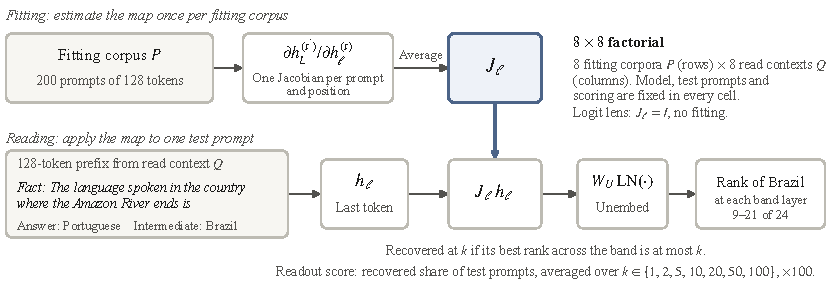
\includegraphics[width=\linewidth]{../figures/fig1_pipeline.pdf}
\caption{The measurement. The fitting corpus $P$ supplies the prompts $J_\ell$ is averaged over
(top); the read-context corpus $Q$ supplies the 128-token passage in front of each test prompt
(bottom). The factorial varies $P$ and $Q$ over eight corpora each, holding all else fixed.}
\label{fig:pipeline}
\end{figure}

% =====================================================================
\section{Related work}

\paragraph{Transport readouts.} A transport readout maps a mid-layer activation to the vocabulary
through a linear surrogate for the layers above it: the identity for the logit
lens~\citep{nostalgebraist2020}, an affine map fitted per layer for the tuned
lens~\citep{belrose2023tuned}, and a layer-skipping map fitted on one named corpus
in~\citet{yomdin2024jump}. The Jacobian lens~\citep{gurnee2026} averages the model's own derivative,
with antecedents and relatives
in~\citet{hernandez2024linearity,geva2022ffn,pal2023future,katz2024backward,szablewski2025transport,liu2026jacobianscopes};
\citet{yan2026shorthorizons} analyse the averaged map's structure. Our question is the distribution it
is estimated over.

\paragraph{Measurement validity.} Unreported analytic flexibility manufactures
findings~\citep{simmons2011falsepositive}, and one defence is to publish the grid of defensible
analyses~\citep{steegen2016multiverse,botviniknezer2020variability,bouthillier2021variance}.
Interpretability scores move under unreported choices~\citep{miller2024faithfulness,zhang2024patching},
apparent structure can trace to the analysis set~\citep{bolukbasi2021illusion,makelov2023illusion},
and mechanistic analysis can be treated as estimation with a variance
budget~\citep{meloux2025estimation,meloux2025identifiable}. Control
tasks~\citep{hewitt2019control,belinkov2022probing}, randomised-network
nulls~\citep{adebayo2018sanity,meloux2025salmon} and construct
validity~\citep{cronbach1955construct,jacobs2021measurement} frame what a readout establishes; a
statistic chosen because it passes its own control is circular~\citep{kriegeskorte2009circular}, and
a successful readout is not a mechanism~\citep{geiger2023abstraction,lin2026identification}.

% =====================================================================
\section{Experimental setup}
\label{sec:setup}

\paragraph{Models and corpora.} We use the Pythia deduped suite: the factorial runs at 410M, the
replications at 1B and 2.8B, and 1.4B is reported descriptively (App.~\ref{app:tables}). At 70M and
160M the fitted lens does not beat the logit lens, so comparisons begin at 410M. Each map is fitted on
$N{=}200$ prompts of 128 tokens unless stated, from one of eight corpora. Five are components of the
Pile~\citep{gao2021pile}, Pythia's training set: English Wikipedia, USPTO patent backgrounds, Pile-CC
web text, StackExchange and GitHub code. Three postdate it or lie outside it: BBC news from June 2024,
arXiv papers from 2023, and Common Pile, an openly licensed collection. We measure how much of each
corpus Pythia saw with \emph{32-gram containment}, the fraction of a corpus's 32-token windows that
occur verbatim in Pythia's published training data, from 0 (none) to 1 (all). GitHub, for example,
scores $0.934$. The five Pile components score above $0.9$ and the three later corpora below
$0.002$, a level reformatting alone can produce: re-wrapping identical text can leave $0.14\%$ of its
32-grams intact. We therefore describe those three as showing no detectable match rather than as
absent from training (App.~\ref{app:data}). Each test prompt is read
at its final token after a 128-token passage from the read-context corpus, disjoint from every
fitting prompt.

\paragraph{Readout score.} Each lens is scored in three steps.
\begin{enumerate}[leftmargin=*,itemsep=0pt,topsep=1pt]
\item At each layer of the band, rank the intermediate among all vocabulary tokens by the lens's
logits, with rank 1 at the top. The band is the source's middle band, 38\% to 92\% of the model's
depth, rounded down and ending below the target layer: at Pythia-410M, layers 9 to 21 of 0 to 23.
\item For a threshold $k$, the prompt counts as recovered if its best rank in the band is at most $k$.
\item The readout score is the fraction of prompts recovered, averaged over the seven thresholds
$k\in\{1,2,5,10,20,50,100\}$ and multiplied by 100.
\end{enumerate}
Thus $k$ is a rank threshold, not a layer. If \emph{Brazil}'s best rank across layers 9 to 21 were
7, the Amazon prompt would be recovered at $k=10$, 20, 50 and 100 but not at 1, 2 or 5, and would
contribute $4/7$ of a prompt. A score of 26 is therefore a mean over seven thresholds, not a success
rate. A prompt with several intermediates counts once per intermediate. Word association sits at the
floor for every lens, the logit lens included, so it cannot separate lenses and scores use the other
five families.

\paragraph{Scoring conventions.} Steps 1 and 2 are the source's own
definitions~\citep{gurnee2026}: this paper audits the published measurement, so it scores that
measurement as published. We call this rule \emph{any-layer} recovery (\mn{} in code and
tables) and treat it as primary. The source summarises over $k$ with an area under the curve in
$\log k$; our flat mean likewise avoids choosing one $k$, and differs from it by $4.3\%$ on identical
ranks (App.~\ref{app:config}). As a sensitivity analysis we report \emph{majority-layer} recovery
(\pe{}), which requires the top $k$ at half or more of the band's layers. Layer-permutation nulls,
which score each map with its Jacobians reassigned to the wrong band layers, give conclusions that
depend on this choice, so no claim rests on them (App.~\ref{app:controls}). The
released prompts end in a trailing space that the tokenizer merges into the next token, so an early
version of our scorer read the wrong token on 157 of 551 prompts. Every result here uses the corrected
scorer (App.~\ref{app:config}).

% =====================================================================
\section{Results}
\label{sec:results}

\subsection{Fitting-corpus identity changes the readout}
\label{sec:corpus}

The fitting corpus changes what the lens reads. Averaged over read contexts, the readout score at
Pythia-410M runs from $22.8$ for the map fitted on GitHub to $26.0$ for the map fitted on
StackExchange, against $19.8$ for the logit lens read without a prefix (Fig.~\ref{fig:grid}). In the $8\times8$ grid the
fitting corpus accounts for $53.4\%$ of the variance among cell means, the read context for $44.6\%$
and their interaction for $2.0\%$ (Table~\ref{tab:variance}). Fitting and reading on the same corpus
confers no detectable advantage, and GitHub is the worst fitting corpus in all five families
(Table~\ref{tab:family}).

Different corpora differ far more than different samples of one corpus. We refit maps on four
disjoint document blocks from each of two sources, Pile-CC and Wikipedia. Under any-layer recovery,
source identity accounts for $0.989$ of the variance among these maps' scores, above the threshold of
$0.70$ fixed in advance. This test and the next were registered under majority-layer recovery, before
any-layer became primary, and pass under it too ($0.972$ here, $22.2$ below). Lexical diversity does
not explain the separation either. Here a \emph{seed} is one of three disjoint blocks of fitting
documents per corpus. The \emph{pooled seed SD} is the root mean square, over corpora, of each
corpus's standard deviation across its seeds; it measures how far a score moves when only the sample
changes. With the fitting prompts matched on type-token ratio, the share of distinct tokens in
a window, the spread between corpora stays at $22.7$ pooled seed SDs, above the pre-registered 20. How the variance splits between fitting corpus and read
context depends on the scoring rule: under majority-layer recovery the shares are $50.7\%$ and
$48.1\%$. That the fitting corpus matters does not depend on it.

Pythia answers only 3 to $6\%$ of the test prompts at top-1 (App.~\ref{app:tables}), and the
intermediates were annotated for much larger models, so the maps might differ only in how they order
noise. Three results argue against that. Every fitted map beats the logit lens, by $4.2$ to $7.1$
points under any-layer recovery when read without a prefix, with seven of eight intervals excluding
zero (Table~\ref{tab:crossover}). Maps fitted on a network whose transformer blocks were
re-initialised read below the logit lens on 3 of 3 corpora (App.~\ref{app:controls}), so the gain
needs the trained computation. And the corpus ordering recurs across five independent families,
disjoint fitting samples, and 1B and 2.8B. These tests exclude random noise but not a systematic
bias: a map that promoted frequent tokens whatever the prompt could also beat the logit lens, need
the trained network and order the corpora stably. The results therefore show that the readout score
is sensitive to the fitting corpus, not that the maps recover concepts Pythia represents; that needs a test set
calibrated to Pythia's competence.

\begin{figure}[t]
\centering
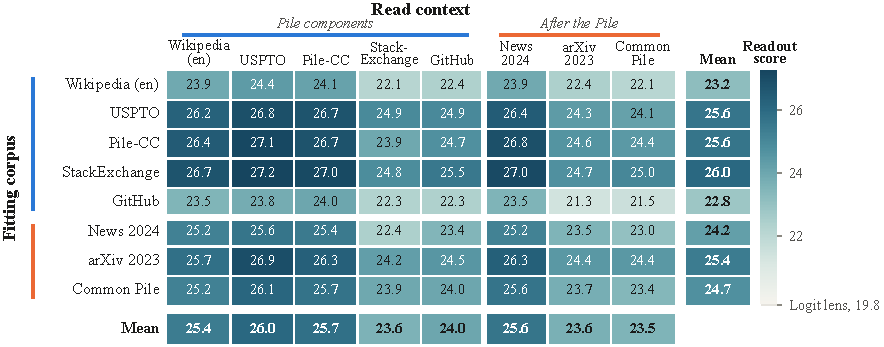
\includegraphics[width=\linewidth]{../figures/fD_grid.pdf}
\caption{Readout score of the $8\times8$ factorial at Pythia-410M under any-layer recovery. Each row
is a map fitted on one corpus; each column is the corpus the read context was drawn from. Model, test
prompts and scoring are identical in all 64 cells. Table~\ref{tab:grid} lists the values.}
\label{fig:grid}
\end{figure}

\subsection{Raw containment does not account for the corpus ordering}
\label{sec:membership}

If maps fitted on corpora Pythia saw more often read better, the three corpora with no detectable
containment should read below the five Pile components. They do not: all three read inside the range
of the five (Fig.~\ref{fig:membership}), and GitHub, the most contained corpus, builds the worst map
of the eight. Raw verbatim containment therefore does not account for the ordering. It is a coarse
proxy for exposure on a panel of eight corpora, so finer exposure mechanisms are not ruled out.

\subsection{The effect replicates at Pythia-1B and 2.8B}
\label{sec:ladder}

At 1B and 2.8B the five Pile corpora were refit, from 200 prompts at 1B and 25 at 2.8B, and compared
with 410M on two criteria fixed before those models were scored (Table~\ref{tab:ladder}). Both use
$z$: the intermediate's logit minus the mean logit over the vocabulary, divided by the logits'
standard deviation, at the band layer where it is largest and averaged over prompts. The spread
criterion requires the between-corpus spread of $z$, best corpus minus worst, to exceed ten pooled
seed SDs ($R\ge10$) in at least four of five families. It is met at both sizes. The agreement
criterion requires Kendall's rank correlation with the 410M corpus ordering, $\tau$, to reach $0.6$
in at least three of five families ($\tau=1$ for identical orderings, $0$ for unrelated ones). It is
met in five of five families at 2.8B and in three of five at 1B. The 1.4B model is reported but not
counted, because its numbers were seen before the criteria were fixed.

\subsection{More prompts do not remove the effect, and no statistic explains it}
\label{sec:unexplained}

As fitting sets grow from 25 to 800 prompts, the largest change in any corpus's readout score is
$0.78$ points, against a spread of $2.46$ points between corpora at fixed $N$ (App.~\ref{app:tables}).
The ratio, $0.32$, misses our pre-registered flatness criterion of $0.25$, so the curves are not
strictly flat, but the corpus matters long after sampling noise has become small beside it. No
statistic we measured identifies which property of a corpus makes its map read better. Of twenty
statistics of the map and the corpus, measured on five corpora, several correlate strongly with the
ordering, such as the dispersion of the per-prompt Jacobians ($r=-0.95$) and the model's
cross-entropy on the fitting corpus ($r=0.83$). Each collapses when one corpus is left out, usually
GitHub, whose removal alone takes those two to $-0.77$ and $0.13$. None of the twenty meets its
criterion (App.~\ref{app:tables}): seventeen faced the leave-one-corpus-out rule fixed in advance,
three a rule on a different unit.

% =====================================================================
\section{Limitations}
\label{sec:limits}

The full factorial was run only at Pythia-410M, the 2.8B maps were fitted from 25 prompts, and
larger models and other model families were not tested. From 410M to 2.8B, top-1 accuracy on the test
prompts stays between 3 and $6\%$ with overlapping intervals (Fig.~\ref{fig:validity}b). The ladder
therefore offers no clean competence axis, and a test set stratified by capability is needed before
extrapolating to the frontier models the lens is meant to audit. With the 128-token prefix every
prompt is read outside positions 16 to 126, where the map was averaged; alignment at the read position
does not order the corpora (App.~\ref{app:controls}), but the evaluation extrapolates in position.
The containment comparison rests on eight corpora and the predictor panel on five, enough to detect a
large effect but not to identify its source. Corpus identity bundles domain, formatting and token
statistics; the band is inherited from the source by proportion; and only read-side recovery is
tested (App.~\ref{app:limits}).

% =====================================================================
\section{Conclusion}

A Jacobian lens depends materially on the corpus its map is fitted on. On Pythia, changing that
corpus alone moves the readout score by more than three points, far more than resampling within a
corpus does, and the dependence recurs at 1B and 2.8B. The lens converges with few prompts, but
convergence to one corpus's map is not invariance across corpora. The fitting corpus should therefore
be reported with the model and layer, and varied as fitting-set size already is.

% =====================================================================
\newpage
% The acknowledgments open the references page, so the body-page gate counts only the body.
\begin{ack}
This work received no external funding and was carried out independently.
\end{ack}

\bibliographystyle{plainnat}
\bibliography{refs}

% =====================================================================
\newpage
\appendix

\section{Additional method details}
\label{app:method}

\paragraph{The estimator decomposition.} Because $J_\ell$ is an expectation under
$P$, the error of a lens fitted on $P$ and used under $Q$ decomposes into a sampling term
$\lVert\hat J^P_N - J^P\rVert$ and a distance term $\lVert J^P - J^Q\rVert$. The usual reading of
``distribution shift'' is that the second drives degradation. Both are relational, and both are
small here. What is large is an absolute property of whichever corpus built the map, which no
relational quantity we computed recovers.

\paragraph{Aggregation definitions.} Any-layer recovery is \mn{} and majority-layer recovery is \pe{}
in code, results files and the generated tables. For band $B$, rank $r_\ell(t)$ of target $t$ at
layer $\ell$, and $K=\{1,2,5,10,20,50,100\}$:
\begin{align*}
\mathrm{score}_{\mn} &= \tfrac{1}{|K|}\sum_{k\in K}\mathbf{1}\!\left[\min_{\ell\in B} r_\ell(t)\le k\right],\\
\mathrm{score}_{\pe} &= \tfrac{1}{|K|}\sum_{k\in K}\mathbf{1}\!\left[\textstyle\sum_{\ell\in B}\mathbf{1}[r_\ell(t)\le k]\ \ge\ \lfloor|B|/2\rfloor\right].
\end{align*}
Both are averaged over target pairs within an evaluation set, then over sets. At $|B|{=}2$, \pe{} degenerates to \mn, so the two aggregations cannot distinguish persistence
behaviour at that band width.

\paragraph{Multi-target items.} These are scored per (item, intermediate) pair, which reduces to the
published formula when every item carries one intermediate and does not reweight items by how many
they carry. The alternatives, counting an item if any or if all of its intermediates are recovered,
are both defensible.

\paragraph{Depth against duration.} The global workspace account predicts \emph{global availability},
that a representation is broadcast to many downstream consumers~\citep{dehaene1998workspace}. The
persistence it describes is temporal and is implemented by recurrence. A transformer's layer index
is not time, and a band of layers is not a duration. Reading a layer band as though depth were time
therefore conflates at least two different objects.

\paragraph{Staged and sustained availability.} A \emph{staged} intermediate is computed at one
depth, consumed, and overwritten: it occupies a few contiguous layers and then is gone. A
\emph{sustained} variable is held across the band while several operations use it. \mn{} counts an item if any band layer recovers the target, so it is the sensitive test for the
staged case; \pe{} asks
whether recovery is sustained across much of the band. Both patterns are scientifically relevant
under a workspace-style reading, and the workspace account does not by itself select either
summary: what it describes is broadcast, causal use and reuse, none of which either statistic
measures. We report \mn{} as primary because it is the published recovery definition, and make no
claim that either summary is uniquely correct.

\paragraph{What a band statistic would have to be matched against.} A statistic is matched to a
construct only once the construct's expected duration across the band has been stated, and no such
duration is stated for this readout. A contiguity-weighted occupancy score, causally validated,
would be one candidate, rewarding a target that stays decodable across adjacent layers. We do not
validate a replacement here; the per-layer ranks one would need are in the released results. A statistic and the null that certifies it are one design decision and should be pre-registered
together (App.~\ref{app:controls}).

\section{Configuration}
\label{app:config}

Released reference implementation, penultimate target layer, $N{=}200$ fitting prompts of exactly
128 tokens, \texttt{skip\_first}${=}16$, \texttt{dim\_batch}${=}128$, fp32, TF32 off, no centering.

\begin{table}[H]
\centering\small
\caption{Differences between the published description, the released implementation, and our
scoring pipeline. The library ships no evaluation code, so every scoring decision is ours. The two
$k$-summaries in the last row differ by $4.3\%$ on identical ranks; within-pipeline comparisons are
unaffected, since everything here is scored under one convention.}
\label{tab:deviations}
\begin{tabular}{@{}lll@{}}
\toprule
Setting & Source & This paper \\
\midrule
Target layer & Penultimate in text, final in code & Penultimate primary, final secondary \\
\texttt{skip\_first} & 0 in text, 16 hardcoded in code & 16, measured immaterial \\
Fitting prompts $N$ & 1000 & 200 \\
Test prompts per family & 50/54/55/52/96/50 in text & Released files: 93/107/55/98/96/102 \\
Readout position & ``The token immediately preceding'' & Last token after stripping, per the data spec \\
Summary over $k$ & Log-$k$ AUC, reported elsewhere & Flat mean over 7 values of $k$ \\
\bottomrule
\end{tabular}
\end{table}

\paragraph{The readout correction.} Section~\ref{sec:setup} states the defect. Its incidence was 157
of 551 items: all 55 order-ops, 83 of 93 multihop, 19 of 107 multilingual, and exactly zero on
poetry, typo and association. Those three untouched sets are the internal control that the two arms
differ in the readout token and in nothing else, and they score identically under both. Every
affected result was re-scored on CPU. The decomposition it moves is the read axis becoming visible
rather than the fit axis weakening, since a bare space cannot see a 128-token prefix.

\paragraph{Choice of the primary aggregation.} \pe{} was adopted as a summary after the
random-derangement comparison and is the aggregation that separates from that null, which would
make it circular as a primary in the sense of~\citet{kriegeskorte2009circular}. \mn{} is the
source's own definition and is primary here for that reason; the corrected-readout decomposition
was computed before that choice was made, and \mn{} is the only aggregation in which the fitting
axis clears zero. The permutation nulls are not used to identify layer correspondence under either
aggregation (App.~\ref{app:controls}).

\paragraph{Scope of the audit.} This paper tests the \emph{calibration} of the
corpus-averaged map: whether the quality reported for a Jacobian lens depends on a fitting
choice that is not reported. It does not test the causal interventions built on that
map~\citep{gurnee2026}, the directed-modulation results, the broadcast experiments, or the
workspace interpretation itself. Those rest on evidence this paper neither reproduces nor contests.
What our results bound is the read a fitted map produces, on one test set, on one model
family.

\paragraph{Agreement with the source.} We adopt the source's own operational definitions rather
than criteria we constructed. The published evaluation defines an intermediate as recovered at $k$
if it appears among the top-$k$ tokens \emph{at any} band layer, and that is the statistic we report
as primary. The source is likewise explicit that the J-space is ``workspace-like'' in an
intermediate band rather than a demonstrated neuronal workspace, and that the boundary between that
band and the output regime was identified empirically. Nothing in this paper disputes either
reading; we test the calibration of the average the map is built from.

\paragraph{The inherited band.} We take the normalised $L38$--$L92$
band by proportion and do not re-identify it on Pythia using the source's own diagnostics, which
rest on functional interventions over tasks the model can perform. Pythia answers 3 to $6\%$ of the
test prompts at top-1 (Table~\ref{tab:competence}), so those diagnostics are unavailable here. The same
competence ceiling caps the answer rate. What our
results require is that the band be \emph{the same} in every cell, not that it be a workspace. It is
identical across all 64 cells of the factorial and is swept from 1 to 13 layers wide on three
corpora (App.~\ref{app:controls}). A one-layer error in it is immaterial. At 1B the corpus-by-set
interaction is $9.19\%$ on $[6,13]$ against $9.16\%$ on $[5,13]$, with the corpus main effect at
$2.24\%$ either way. The band's location is inherited; the conclusions drawn inside it are
not conditional on that location being correct.

\section{Dataset and evaluation protocol}
\label{app:data}

Our containment index follows~\citet{marone2023portraits,elazar2024wimbd,oren2024contamination}, and
\citet{lee2022dedup,carlini2021extracting,biderman2023memorization} inform our separation of
membership from verbatim recurrence. Each corpus supplies windows of exactly 128 tokens drawn from
disjoint document pools per seed block. Licensed plaintext is not redistributed; we ship the
builder, a manifest of per-file hashes, and item identifiers.

\tblcontain
\tblcalib

\begin{figure}[H]
\centering
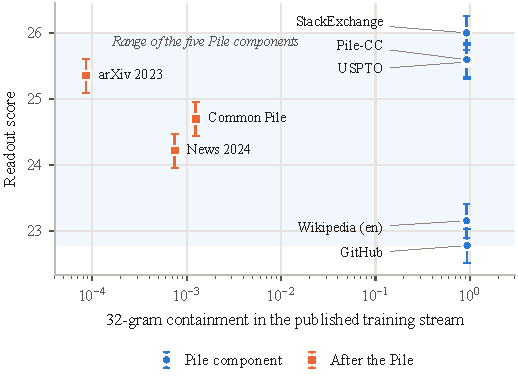
\includegraphics[width=0.72\linewidth]{../figures/fM_membership.pdf}
\caption{32-gram containment against Pythia's published training data, on a log axis, against the
any-layer readout score each fitting corpus produces, averaged over the eight read contexts. The
shaded band is the range of the five Pile components; all three later corpora fall inside it, and
the worst map of the eight, GitHub, has containment $0.934$. Error bars are the pooled seed SD;
Spearman $-0.10$ over eight corpora.}
\label{fig:membership}
\end{figure}

\paragraph{Contamination and overlap.} Read-context pools were verified disjoint from every fitting
pool; without that step, roughly a quarter of a diagonal cell's context documents would be documents
its own map was fitted on. One out-of-stream corpus is $33.4\%$ exact duplicates, and
deduplicating and refitting moves its read in the direction that weakens the reported contrast. The read-context dose sweep of App.~\ref{app:tables} predates that disjointness step and carries a
measured $17.0\%$ overlap on its diagonal cells, a second reason it is not used as evidence; the
factorial's pools are disjoint.

\section{Additional results and ablations}
\label{app:tables}

\paragraph{The twenty candidate predictors.} From the map's spectrum and geometry: three
dispersion statistics, stable rank, top-8 spectral share, condition number, alignment to the
identity, cross-layer cosine. From corpus statistics: prompt length, type-token ratio,
evaluation-vocabulary overlap, model cross-entropy. From this paper's own instruments: the
activation- and read-space distances, disagreement geometry, concept-conditional activation energy.
Seventeen are tested at $n{=}5$ corpora against the $|r|\ge0.8$ leave-one-corpus-out rule; three sit
on a different unit under a different criterion. None of the twenty meets its own criterion.

\paragraph{The ablation inventory.} Each manipulation below varies one design choice and asks
whether the result survives. Dropping corpora leaves the fit-over-read ordering in 6 of 8
single drops and 20 of 28 pairs, at a $21.0\%$ fit share on the worst split. An independent
$5\times5$ grid of $N{=}400$ maps refitted by a different code path gives $67.2$ against $30.9$
under \mn{} and reverses under \pe. Matching the fitting
pools on type-token ratio grows the spread from $16.0$ to $22.7$ seed SD under \mn{} and shrinks it
from $30.1$ to $22.2$ under \pe, with the matching control at $11.1\%$ against a $10\%$ bar.
Varying $N$ over a $32\times$ range moves the readout score by at most $0.78$ points per corpus,
against a between-corpus spread of $2.46$ points at fixed $N$. The pre-set criterion for calling that curve flat
required the ratio to fall below $25\%$; it reached $31.9\%$, so the criterion was not met cleanly.
A read-context dose sweep over prefixes of 128, 384 and 768 tokens exists in the stored record but
was scored under the pre-correction readout. Four independent lines establish this: no corrected
flag in its recorded invocation, a script hash matching the pre-fix scorer, no readout key in its
payload, and dose-128 row means within $0.05$ points RMS of the legacy factorial against $11$ points from
the corrected one. It is therefore not counted among the checks above. At the 128-token prefix the
corrected factorial restricted to the same seven corpora gives fit and read shares of $57.6\%$ and
$40.2\%$ under \mn{}, where the legacy sweep gave $77.9\%$ and $19.3\%$. The corrected 384- and
768-token points have not been run, so the corrected dose trend is unresolved.
Every table below is
generated from the stored results files at build time by \texttt{paper/tools/make\_audit\_tables.py},
not transcribed.

\tblvariance
\tblladder
\tblbaseline
\tblfamily
\tblcompetence
\tblposition
\tblcrossover
\tblgrid


\section{Controls and failure cases}
\label{app:controls}

\paragraph{Layer-permutation nulls.} The fitted maps were scored against layer-deranged copies of
themselves, in which every band layer receives another layer's Jacobian under a random derangement. That construction preserves every entry, norm and
spectrum, but it changes two things at once: a layer's correspondence with its own derivative, and
the dependence between layers. \mn{} is an existential aggregation over the band, and the
probability of such a union depends on that dependence, so a comparison against a random
derangement does not isolate correspondence. A pre-registered comparison rescored the same 24
maps against a second null family, the twelve non-trivial cyclic shifts of the band, which
also remove every layer's own Jacobian, under four band summaries: \mn, \pe, the best single layer,
and the band mean. Its gate reproduced every stored corrected arm to $0.00\mathrm{e}{+}00$.
Table~\ref{tab:da1} gives the corpus-clustered paired $t$ on the per-corpus gap. Under \mn{} the
real map beats the cyclic shift on 8 of 8 corpora and loses to the random derangement on 7 of
8. Under \pe{} and the band mean it beats both nulls on 8 of 8 corpora, on all 96 cyclic cells and
all 120 derangement draws. The best single layer is mixed: ahead of the shift on 8 of 8 and
indistinguishable from the derangement. Two nulls that both remove absolute correspondence give opposite conclusions under \mn, so the
conclusion depends on the aggregation and on the null's cross-layer dependence, and neither permutation null
isolates correspondence under \mn. Neither is used as an identifying control, and no claim in the
body rests on them.

The cyclic shift is not a dependence-preserving control either. The mean off-diagonal correlation
of the per-layer recovery events is $0.436$ for the real map, $0.337$ for the cyclic shifts
and $0.328$ for the derangement, so the shift restores about $8\%$ of the dependence the
derangement removes. The two nulls differ in how far each sits from the independent-layer prediction of the union, one
axis \mn{} is sensitive to and the band mean is not. Because a cyclic
shift changes only which band activation meets which Jacobian, the band-mean and \pe{} results are
evidence that the pairing carries information, and that statement is not selected on the control
it must pass: the band mean was defined before any derangement result existed. A further
exploratory comparison gives every band layer the band-average map. Under \pe{} that single average matches the layer-specific map, $10.80$ against $10.78$ points
with the free lens at $8.32$, while under \mn{} the real map is ahead on 8 of 8. The average is a different object
with a different norm and spectrum, so this is not a matched control and supports no conclusion.

\begin{table}[H]
\centering\scriptsize\setlength{\abovecaptionskip}{2pt}\setlength{\belowcaptionskip}{4pt}\setlength{\tabcolsep}{4pt}
\caption{The fitted maps against two layer-permutation nulls under four band summaries, corrected
readout, 410M. Each cell gives the mean per-corpus gap in readout-score points (real minus null), the
corpus-clustered paired $t(7)$, and the number of corpora on which the real map is ahead. The
cyclic-shift row averages the twelve non-trivial shifts and the derangement row the fifteen draws
of Table~\ref{tab:derange}.}
\label{tab:da1}
\begin{tabular}{@{}lllll@{}}
\toprule
Null & Any-layer (\mn) & Majority-layer (\pe) & Best single layer & Band mean \\
\midrule
Cyclic shift & $+1.6$, $t{=}7.70$, 8/8 & $+2.7$, $t{=}15.8$, 8/8 & $+1.1$, $t{=}4.59$, 8/8 & $+2.4$, $t{=}25.6$, 8/8 \\
Random derangement & $-0.5$, $t{=}-1.92$, 1/8 & $+2.8$, $t{=}17.5$, 8/8 & $+0.1$, $t{=}0.58$, 4/8 & $+2.3$, $t{=}25.9$, 8/8 \\
\bottomrule
\end{tabular}
\end{table}

\tblderange
\tblclustered

\begin{figure}[H]
\centering
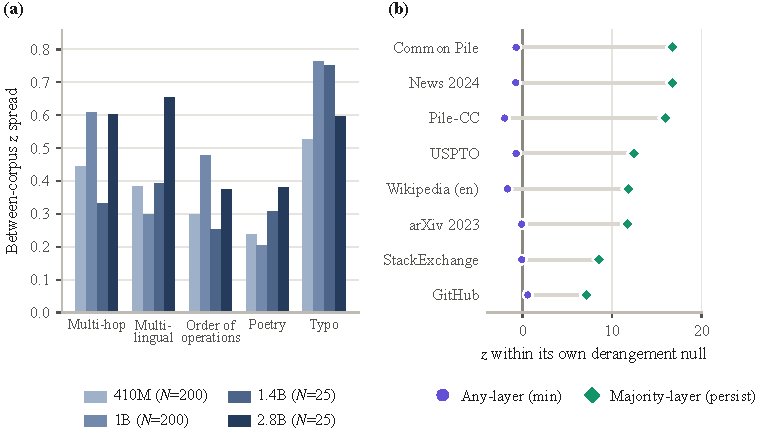
\includegraphics[width=0.95\textwidth]{../figures/fA_effect_and_null.pdf}
\caption{(a) Between-corpus $z$ spread at four ladder rungs, which is the panel
Section~\ref{sec:ladder} cites. The spread, not $R$, is what compares across rungs, since $R$'s
denominator moves with the fitting sample size $N$ printed in the legend. (b) Each map scored
against fifteen layer-deranged copies of itself, in units of its own null's SD, under both
aggregations. Panel (b) is recorded under the qualification at the head of this section: a random
derangement changes cross-layer dependence as well as layer correspondence, so we do not read it as
an identifying control, and no claim in the body rests on it.}
\label{fig:effect}
\end{figure}

\begin{figure}[H]
\centering
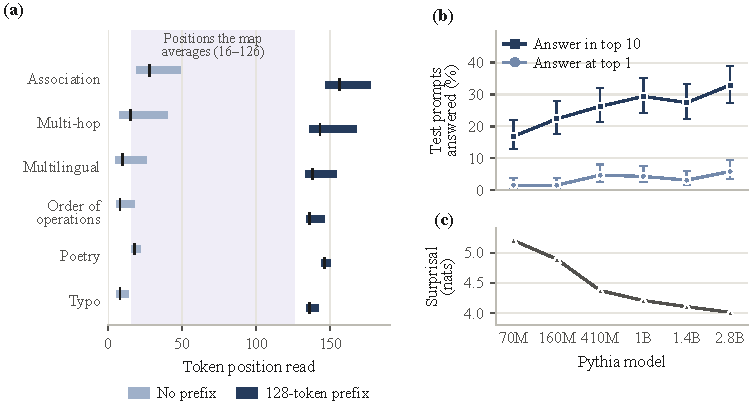
\includegraphics[width=0.95\textwidth]{../figures/fB_validity.pdf}
\caption{(a) The Jacobian is averaged over positions 16 to 126, shaded. With a 128-token prefix no
test prompt in any of the six families is read inside that window; without a prefix most families
sit below it. (b) The share of test prompts whose answer the model ranks first, or in its top 10, up
the Pythia ladder, with 95\% Wilson intervals: top-1 never separates from 410M. (c) Mean prompt
surprisal, which falls throughout.}
\label{fig:validity}
\end{figure}

\paragraph{Read position and the extrapolation test.} The map averages a per-position Jacobian
over positions 16 to 126 of a 128-token window. With the 128-token read prefix the test prompts' readout
tokens sit at positions 133 to 177, median 142, so $0$ of $551$ items are read inside the fitted
range. Without a prefix $45.7\%$ are, the rest falling below 16 in the attention-sink zone the
fitter excludes (Fig.~\ref{fig:validity}a; Table~\ref{tab:position}, App.~\ref{app:tables}). The
evaluation therefore tests extrapolation, in opposite directions under the two conditions.
Extrapolation does not appear to order the corpora. The reference transport $G_\ell(p)$ is the
position-$p$ slice of the released estimator, averaged over 128 held-out prefixed sequences and
independent of which corpus any map was fitted on. Alignment at the median read position does
not order the corpora the way the readout does, at Spearman $\rho=+0.143$ against a critical
$|\rho|$ of $0.714$ at $n{=}8$, exact two-sided $p=0.752$. A GitHub-built probe gives
$\rho=-0.048$ at $p=0.935$, so the null does not depend on the probe's corpus. All five controls are met. The Frobenius
cosine is scale-invariant to $4.8\times10^{-11}$ against a $10^{-9}$ bound. In-support alignment is
at least $0.794$ for all eight corpora against a bar of $0.30$, while alignment against a
norm-matched Gaussian is at most $2.0\times10^{-4}$ against a bar of $0.05$, so the metric is not
vacuous. The 128 items building $G$ and the 270 scored are disjoint. The probe position 142 lies inside the
measured prefixed read range $[133,177]$, and the band equals the asserted rule. A
descriptive oracle read was planned and not executed.

\paragraph{Two controls on the corpus-identity row.} The composition control of
Section~\ref{sec:corpus} required the post-matching spread to fall below $10\%$ of the pre-matching
spread and reached $11.1\%$, so that row is reported with its bar unmet. The map-space contrast
is separately recorded inconclusive, on the map-space control below.

\paragraph{The choice of $z$.} Section~\ref{sec:ladder} and Table~\ref{tab:ladder} measure the scale
replication in $z$, the standardised logit defined there. Against a layer-deranged control the units
are not interchangeable: $z$ slightly favours the real map and rank and margin do not. That
comparison carries the same qualification as the permutation nulls above.

\ifdefined\EXTENDED
\paragraph{Score units.}\label{app:scoreunits} A pre-registered check asks whether the corpus effect is
an artifact of scoring by rank, which can move a target past many near-tied tokens without the lens
scoring it higher. It ran before submission, and its primary result is reported only in this extended
version. It measures the between-corpus spread at 410M, on the five Pile corpora and 801 scored pairs, in
three units, each divided by its own pooled seed SD. In rank, as in the readout score, the spread is
$9.4$; in the margin, the target's logit minus the best competing token's, it is $23.1$; in $z$ it is
$27.2$. The
pre-registered statistic, the margin ratio over the rank ratio, is $2.46$. The rule fixed in advance
called a value of at least $0.50$ a score effect and a value below $0.25$ a ranking artifact, so the
verdict is a score effect: fitting-corpus sensitivity is not confined to rank-based scoring. This does
not resolve the competence objection of Section~\ref{sec:corpus}. A map can raise a target's logit
without the model representing the concept, and only a test set calibrated to Pythia's competence
would settle that.
\fi

\begin{figure}[H]
\centering
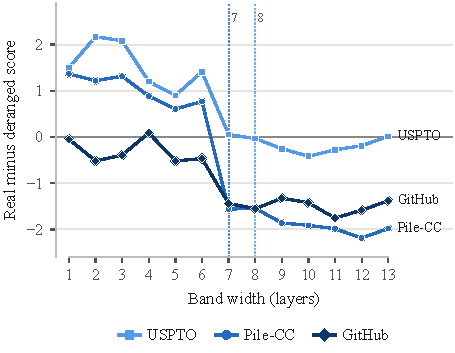
\includegraphics[width=0.62\textwidth]{../figures/fU_union.pdf}
\caption{Real minus layer-deranged readout under \mn{} as the band is widened from 1 to 13 layers.
The deranged map overtakes the real one at width 7 on Pile-CC and 8 on USPTO, while GitHub sits at
or below its derangement at 12 of 13 widths, including width 1, where no union can operate. The
sweep is evidence that union inflation contributes to the \mn{} result on two corpora, not a
complete account of it. The source's band is 13 layers wide at 410M.}
\label{fig:union}
\end{figure}

\paragraph{The width sweep.} Three clauses would together describe a union mechanism. Two hold on
all three corpora tested. The third, that the derangement is worse at individually more band layers,
holds on two of three: it is lower at 12 of 13 layers on USPTO and GitHub and at 11 of 13 on
Pile-CC. The sweep therefore supports union inflation as a contributor to the \mn{} result on
Pile-CC and USPTO and does not account for GitHub, which sits below its derangement at width 1.

\paragraph{The randomised-network null.} Re-initialising every transformer block from the model's
own initialiser, holding the embedding, unembedding and final norm fixed, destroys the computation
while leaving the readout path real. Cross-entropy rises to $11.85$--$14.29$ nats against a
gate of $8.0$. Maps refitted on that network read below the free logit baseline on 3 of 3 corpora, closest
approach $-2.45$ points against a baseline of $2.84$. Both aggregations floor it,
so this control does not discriminate between them. The obvious implementation is a silent no-op on
recent library versions, because the initialisation flag is stamped on the tensor and the
re-initialiser skips it; our fitter clears the flag and aborts if the block Frobenius norm does not
move.

\paragraph{Variance of a single derangement draw.} Across 20 random derangements at 410M over
a 13-layer band, the number of evaluation sets the real map wins has mean $1.5$ to $3.3$ and
standard deviation $0.67$ to $1.03$ under \mn, and mean $3.1$ to $4.9$ with standard deviation
$0.22$ to $0.50$ under \pe. A single-draw win count is therefore a draw from a distribution roughly
one set wide, which is why the aggregation gradient is reported as an ordering rather than as exact
counts. The same study separates two explanations this record otherwise cannot. At 70M the band rule gives
2 layers, so $\lfloor|B|/2\rfloor=1$ and \pe{} \emph{is} \mn. There the real map wins all 6
sets in every one of 20 draws, with zero variance. ``Small models are different'' and ``narrow
bands are different'' are observationally identical here.

\paragraph{The scale floor and the raw unembedding geometry.} At 70M and 160M the fitted lens
does not improve on the unfitted baseline under this evaluation, so the main comparison starts at
410M. Statistics of the raw, uncentred concept rows of $W_U$ differ sharply below 410M. Mean pairwise
cosine is $0.959$ and $0.922$ at 70M and 160M against $0.031$ and $0.020$ at 410M and 1B. The
number of directions carrying $90\%$ of the spectral energy is 1, 1, 371 and 508, and a
Roy--Vetterli entropy rank gives $199.1$, $368.6$, $725.9$ and $969.3$. A single additive direction
common to every row can dominate all of these while cancelling out of the rank comparison the
readout performs, so they do not identify the cause of the small-model floor, which is not
explained here.

\paragraph{Map-space control.} The map-space contrast is inconclusive because one of its five
controls, C1, required exactly zero from two self-distance metrics. On the scale-free relative
distance $d_{\mathrm{rel}}(A,A)$ is exactly $0.0$ for every one of the 24 maps in float32, so that
half of C1 is met. On the mean principal angle it is not: the float32 floor is $4.432\times10^{-4}$
against a predicted $\sqrt{2\varepsilon_{32}}=4.883\times10^{-4}$, it collapses to
$1.732\times10^{-8}$ in float64, and a norm-matched random matrix reproduces it at
$3.519\times10^{-4}$. The pre-registered rule for setting C1 aside applies only if its conditions hold on both metrics,
and a metric returning an exact zero leaves no floor for a random matrix to reproduce, so the
contrast stays inconclusive. The primary contrast and the other three gated controls are
unaffected.

\section{Reproduction}
\label{app:repro}

Code, pre-registrations and documentation: \url{https://github.com/tarush-ai/fittingcorpus}.
Results files and fitted maps: \url{https://huggingface.co/Tarush-AI/fittingcorpus}.
The code repository carries every pre-registration with its decision rule, an experiment registry
and the reproduction harness. The Hugging Face repository carries every results file and every
fitted map, and the code repository lists each of those files with its hash. Corpus plaintext is
third-party text, so it is rebuilt from its public sources at pinned dataset revisions and checked
against per-file hashes rather than redistributed.

\paragraph{Tiers.} Reproduction is organised in three tiers that answer different questions. At
tier T0 every statistic in this paper is recomputed from the stored results files, on a laptop, in
about a minute. All 15 T0 modules run, and 14 recompute a payload identical to the stored one. The
fifteenth differs only in the recorded hash of a pre-registration whose wording changed after the
run; its receipt is in the code repository. At tier T1 every read is
re-scored from the stored maps on CPU. A sweep of the 22 T1 modules that existed at submission
reproduced every scientific quantity, 16 of them bit for bit, the other six differing only in a
recorded file path or timing field; the harness now has 31 T1 modules. At tier T2 maps are refit
from the corpora on a GPU in fp32 with TF32 off; two refits were run as implementation checks,
chosen to straddle the date the provenance layer was added, and they are not a statistical
replication. Corpora are byte-identical to their manifests (11 of 11), recorded map input hashes
still match on disk (385 of 385), and recorded payload hashes are unmoved (92 of 92).

\paragraph{Reproduction note.} One historical eight-corpus panel of maps predates the provenance
layer and refits to a maximum element difference of $1.1\times10^{-3}$, above the single fp16
storage step its values allow. The fitter's measured determinism floor is about $10^{-6}$, so the
gap is real and is attributed to machine and library state that was not recorded. It does not
affect any readout. A fresh refit and the stored map give reads that differ by exactly $0.0$ under
both aggregations, and a perturbation of the same magnitude moves the read by about a tenth of a
seed standard deviation. A map fit after the provenance layer was added refits to within one fp16
step. The comparison is recorded in the code repository.

\paragraph{Decision rules and audit.} The code repository carries every experiment's pre-registered
decision rule, its controls with the value that would make each fail, the readout-correction ledger,
a ledger of whether each pre-registration was committed before its code, and the record of the T1
sweep. The working files of the internal audits are not released.

\section{Broader impact and responsible use}

This work analyses openly released model weights and openly released or licensed text. It produces
no model, no capability uplift and no data release, and involves no human subjects or personal data.

\paragraph{The dual-use component.} Our containment index queries candidate corpora
against a published training stream, which is the same primitive as a membership-inference attack.
Three things bound the risk. It is applied only to public corpora and never to text identifying a
person. It is applied only to a model that publishes its training stream, so no inference is needed
to learn what that model saw. And its resolution is deliberately coarse: whole-corpus containment at
$k{=}32$ rather than per-document membership decisions, in a regime where the index cannot separate
absence from reformatting.

\paragraph{Relevance of the negative results.} Transport readouts are proposed
for auditing and oversight, a setting where a confident wrong answer is worse than no answer. In the method studied here, the measured quality of the readout is governed substantially by a
fitting corpus that the original evaluation does not vary. Two groups running the same method
on the same model can therefore obtain results differing by more than the effects they are studying. And the published aggregation
statistic, read against a layer-permutation null, returns a conclusion that depends on which null is chosen, so a structural control has to be designed together with the statistic it certifies.
Neither finding says the method is wrong. Both say that a readout used as evidence about a model should ship with its fitting corpus and a
matched structural control.

% =====================================================================
\section{Limitations and future work}
\label{app:limits}

\subsection{Where the evaluation sits}

All eight corpus-fitted lenses outperform the unfitted logit lens at 410M under both aggregations
(Table~\ref{tab:crossover}). Under \mn{} the readout scores run $24.05$ to $26.93$ points against
$19.81$ for the logit lens; under \pe{} the gain is $17.7$ to $44.3\%$. Table~\ref{tab:crossover}
scores each lens on the test prompts read without a corpus prefix and averages over five families and
three seeds, whereas Figure~\ref{fig:grid} averages each map over eight prefixed read contexts. The top-ranked
corpus therefore differs between them, arXiv 2023 there and StackExchange here, while GitHub is
last in both. Seven of the eight \mn{}
differences and two of the eight \pe{} differences have bootstrap intervals excluding zero. This is
measured where the model answers $4.7\%$ of the test prompts at top-1 and places the answer in the top
ten $26.3\%$ of the time (Table~\ref{tab:competence}).

In the Qwen replication of~\citet{nanda2026review} the lens lost to an answer-swap baseline on a
task the model could already do, where the annotated intermediate is close to the obvious
continuation; that observation motivates the capability-stratified test set below. At 70M and 160M
the fitted lens does not improve on the unfitted baseline under this evaluation, which is why the
main comparison starts at 410M; that floor is not explained here (App.~\ref{app:controls}).

Whether the fitted lens degrades as capability rises is not identified here. Every top-1 interval
from 410M to 2.8B overlaps every other, so the ladder supplies no clean top-1 competence gradient to correlate a readout against.

\subsection{Limitations}

Beyond Section~\ref{sec:limits}: a corpus is a factor, not an explanation, since it bundles
formatting, boundaries, token frequencies and surprisal, and the five-corpus predictor screen
cannot identify which of these orders the readout. The band is inherited from the source by
proportion; a one-layer error in it is immaterial to these conclusions (App.~\ref{app:config}),
but whether it is the workspace band for Pythia is not tested. The map-space contrast stands
inconclusive because one registered control could not be met on one of its two metrics
(App.~\ref{app:controls}). The small-model floor at 70M and 160M is measured and not explained.
That the lens recovers a latent workspace~\citep{dehaene1998workspace} in Pythia is not supported
on this test set, and this paper reports read success only; write-side steering through the same
map is untested.

\subsection{Future work}

A capability-calibrated, Pythia-native test set with annotated intermediates, read inside the fitted
positional support, would separate readout variation from readout noise, make the source's own
band diagnostics available on this model family, and supply the competence axis this ladder lacks.
A larger corpus panel, with controlled manipulations of entropy, repetition, formatting and domain
that hold the rest of the text fixed, would test which bundled property of a corpus drives the
ordering. Another fitted lens, the tuned lens in particular, would test whether fitting-corpus
dependence is a property of fitted transports in general, which a fitting-driven account predicts
and the unfitted logit lens cannot show. And write-side steering and causal interventions through
the same map would test whether fitting-corpus dependence changes the conclusions drawn from the
lens, not only its readout score.

\section{Use of AI assistance}

LLM-based assistants were used under author direction: Claude Opus 5 and Claude Fable 5 for code
implementation, debugging, analysis scripts and the reproduction harness; alphaXiv for literature
search; and LLM assistants for manuscript drafting and revision. Experimental design,
pre-registered decision rules, controls, interpretation, source verification, and final
responsibility for all claims remained with Tarush Gupta.

\end{document}
